\documentclass[unicode,aspectratio=43]{beamer}
\usetheme{Moscow}

\usepackage[utf8]{inputenc}
\usepackage[T2A]{fontenc}
\usepackage[main=russian,english]{babel}
\usepackage{tikz}
\usepackage{movie15}
\usepackage{animate}

\usepackage{caption}

\usepackage{graphicx}

%%%%%%%%%%%%%%%%%%%%%%%%%%%%%%%%%%%%%%%%%%%%%%%%%%%%%%%%%
\def \ve{\varepsilon} % USE
\def \eps{\epsilon}
\def \del{\delta}
\def \ved{{\varepsilon,\del}}%
\def \KSD{\K^{\star, \delta}}
\def \lm{\lambda}
\def \Lm{\Lambda}
\def \la{\left\langle\rule{0pt}{3em}}
\def \ra{\right\rangle}
\def\mx{\mathsf m}
\def\fr{\mathsf f}
%%%%%%%%%%%%%%%%%%%%%%%%%%%%%%%%%%%%%%%%%%%%%%%%%%%%%%%%%
\newcommand{\Ab}[1]{(A.#1)}
%%%%%%%%%%%%%%%%%%%%%%%%%%%%%%%%%%%%%%%%%%%%%%%%%%%%%%%%%
\def\red{\textcolor{red}}
%%%%%%%%%%%%%%%%%%%%%%%%%%%%%%%%%%%%%%%%%%%%%%%%%%%%%%%%%
\def \gr{\nabla}
\def \pt{\partial}
\def \ptt{\partial_t}
\def \dv{\mbox{$\mbox{div}$}}
\def \div{{\rm div}\,}
%\def \to{\rightarrow}
\def \tow{\rightharpoonup}
%%%%%%%%%%%%%%%%%%%%%%%%%%%%%%%%%%%%%%%%%%%%%%%%%%%%%%%%%
\def \eqdef{\stackrel {\rm def} {=}}
\def \ds{\displaystyle}
%%%%%%%%%%%%%%%%%%%%%%%%%%%%%%%%%%%%%%%%%%%%%%%%%%%%%%%%%
\def \R{{\mathbb R}} \def \C{{\Bbb C}} \def \Z{{\Bbb Z}}
\def \I{{\Bbb I}} \def \N{{\Bbb N}} \def \K{{\mathbb K}}
\def \bs{\boldsymbol}
\def \fr{\mathsf f}
\def \ge{\mathfrak{g}}
%%%%%%%%%%%%%%%%%%%%%%%%%%%%%%%%%%%%%%%%%%%%%%%%%%%%%%%%%


\usepackage{amsmath,amssymb}

\hypersetup{
	pdfauthor={Vitaly Mazepov}
}

%\renewcommand{\thefootnote}{\fnsymbol{footnote}}
\usepackage{euler}
\usepackage{multirow}
\renewcommand*{\arraystretch}{1.2}

\graphicspath{{images/}}
\newcommand{\colorhref}[2]{\href{#1}{\textcolor{miptbase!30!black}{#2}}}

\newcounter{citenum}
\newcommand{\newtotcounter}[1]{}
%%% Реализация библиографии встроенными средствами посредством движка bibtex8 %%%

%%% Пакеты %%%
\usepackage{cite}                                   % Красивые ссылки на литературу


%%% Стили %%%
\bibliographystyle{../BibTeX-Styles/utf8gost71umod}    % Оформляем библиографию по ГОСТ 7.1 (ГОСТ Р 7.0.11-2011, 5.6.7)

\makeatletter
\renewcommand{\@biblabel}[1]{#1.}   % Заменяем библиографию с квадратных скобок на точку
\makeatother
%% Управление отступами между записями
%% требует etoolbox 
%% http://tex.stackexchange.com/a/105642
%\patchcmd\thebibliography
% {\labelsep}
% {\labelsep\itemsep=5pt\parsep=0pt\relax}
% {}
% {\typeout{Couldn't patch the command}}

%%% Цитирование %%%
\renewcommand\citepunct{;\penalty\citepunctpenalty%
    \hskip.13emplus.1emminus.1em\relax}                % Разделение ; при перечислении ссылок (ГОСТ Р 7.0.5-2008)


%%% Создание команд для вывода списка литературы %%%
\newcommand*{\insertbibliofull}{
\bibliography{../biblio/othercites,../biblio/authorpapersVAK,../biblio/authorpapers,../biblio/authorconferences}         % Подключаем BibTeX-базы % После запятых не должно быть лишних пробелов — он "думает", что это тоже имя пути
}

\newcommand*{\insertbiblioauthor}{
\bibliography{../biblio/authorpapersVAK,../biblio/authorpapers,../biblio/authorconferences}         % Подключаем BibTeX-базы % После запятых не должно быть лишних пробелов — он "думает", что это тоже имя пути
}

\newcommand*{\insertbiblioother}{
\bibliography{../biblio/othercites}         % Подключаем BibTeX-базы
}


%% Счётчик использованных ссылок на литературу, обрабатывающий с учётом неоднократных ссылок
%% Требуется дважды компилировать, поскольку ему нужно считать актуальный внешний файл со списком литературы
\newtotcounter{citenum}
\def\oldcite{}
\let\oldcite=\bibcite
\def\bibcite{\stepcounter{citenum}\oldcite}

\renewcommand{\citepunct}{,\,}

\title[Задача Римана о распаде разрыва]{Вычислительные алгоритмы, основанные на решении обобщенной задачи Римана}
\date{30 мая 2018, МФТИ, Долгопрудный}
\author[Мазепов Виталий]{\textbf{Мазепов Виталий}\\[1ex]
	Специальность 03.04.01 -- Прикладная математика и физика \\[1ex]
	Научный руководитель:\\
	кандидат физико-математических наук,\\
	\textbf{Скалько Юрий Иванович}}
\institute[МФТИ]{Московский физико-технический институт}

\newcommand{\Ip}{\mathrm{\mathit{I}}_\text{p}}
\renewcommand{\vec}[1]{\boldsymbol{\mathbf{#1}}}
\newcommand{\pd}[2]{\frac{\partial #1}{\partial #2}}
\let\dividesymbol\div
\renewcommand{\div}{\operatorname{div}}
\newcommand{\grad}{\operatorname{grad}}

\begin{document}
\begin{frame}[plain]
\maketitle
\end{frame}

\begin{frame}[plain]

\tableofcontents
\end{frame}

\section{Введение}

\subsection{Общая характеристика работы}

\begin{frame}\frametitle{Актуальность}
\begin{itemize}

\item	Многие эволюционные процессы моделируются гиперболическими системами линейных дифференциальных уравнений первого порядка
	
\item	При построении численных алгоритмов решения краевых задач для таких систем уравнений ключевым моментом является решение задачи Римана
	
\item	В случае многих пространственных переменных методы, основанные на наличии характеристик, уже не работают
	
\item	Предложенный алгоритм сводит задачу нахождения значений переменных в момент
времени $t > 0$ по обе стороны от разделяющей поверхности к решению
системы алгебраических уравнений
\end{itemize}
\end{frame}


\begin{frame}\frametitle{Цели работы}
	\textit{Скалько Ю.И.} Задача Римана о распаде разрыва в случае многих пространственных переменных // Труды МФТИ --- 2016 --- Т. 8., \textnumero 4 --- С. 169-182
	\begin{itemize}
	\item Построить вычислительный алгоритм решения начально-краевой задачи для гиперболической системы линейных дифференциальных уравнений 1 порядка в случае многих пространственных переменных на основании приведенного в статье решения задачи Римана
	\pause
	\item Верифицировать полученный алгоритм
	\item Применить построенный численный алгоритм для ряда прикладных задач
	\end{itemize}
\end{frame}

\section{Основная часть работы}
\subsection{Теория решения обобщенной задачи Римана}

%\begin{frame}\frametitle{Постановка задачи}
%\animategraphics[loop,controls,width=\linewidth]{6}{elastic-}{0}{40}

%\end{frame}
\begin{frame}\frametitle{Обобщенная задача Римана}
	
	\begin{equation*} \label{eq:1}
	\frac{{\partial {\mathbf{u}}\left( {t,{\mathbf{x}}} \right)}}{{\partial t}} +
	\sum\limits_{i=1}^N {{\mathbf{A}_i} \frac{{\partial {\mathbf{u}}\left( {t,{\mathbf{x}}}
				\right)}}{{\partial {x_i}}}}  = {\mathbf{0}},\quad {\mathbf{x}} \in {R^N}
	\end{equation*}
	
	Начальные условия: $ \mathbf{u} (0,\mathbf{x})  = \mathbf{u}_0 (\mathbf{x}) $
	\pause
	Условия сопряжения: 
	\begin{equation*} \label{eq:3.3}
	\mathbf{L} ( \mathbf{u} (t, \mathbf{x} \in \Gamma^-), \mathbf{u} (t, \mathbf{x}\in \Gamma^+) ) = {\mathbf{0}}		
	\end{equation*}
	
	\begin{itemize}
		\item Условия сопряжения отражают физические условия, которые необходимо выполнять на границе  $ \Gamma $. 
		\item 	Начальные данные по обе стороны от гиперплоскости $\Gamma$  могут быть произвольными непрерывными функциями, подчиняющимися условиям сопряжения. 
	\end{itemize}
	
\end{frame}


\subsection{Построение вычислительного алгоритма}


\begin{frame}\frametitle{Решение обобщенной задачи Римана}
	В работе приведен алгоритм для численного решения начально-краевой задачи для гиперболической СЛДУ. Этот алгоритм включает 2 этапа:
	\begin{itemize}
		\item нахождение решения на границе $\Gamma$
		\item нахождение решения в произвольной точке
	\end{itemize}
\end{frame}	

\begin{frame}\frametitle{Решение обобщенной задачи Римана}
	\begin{figure}[ht!]
		\centering
		\begin{minipage}{0.5\textwidth}
	\begin{figure}[ht!]
		\centering
		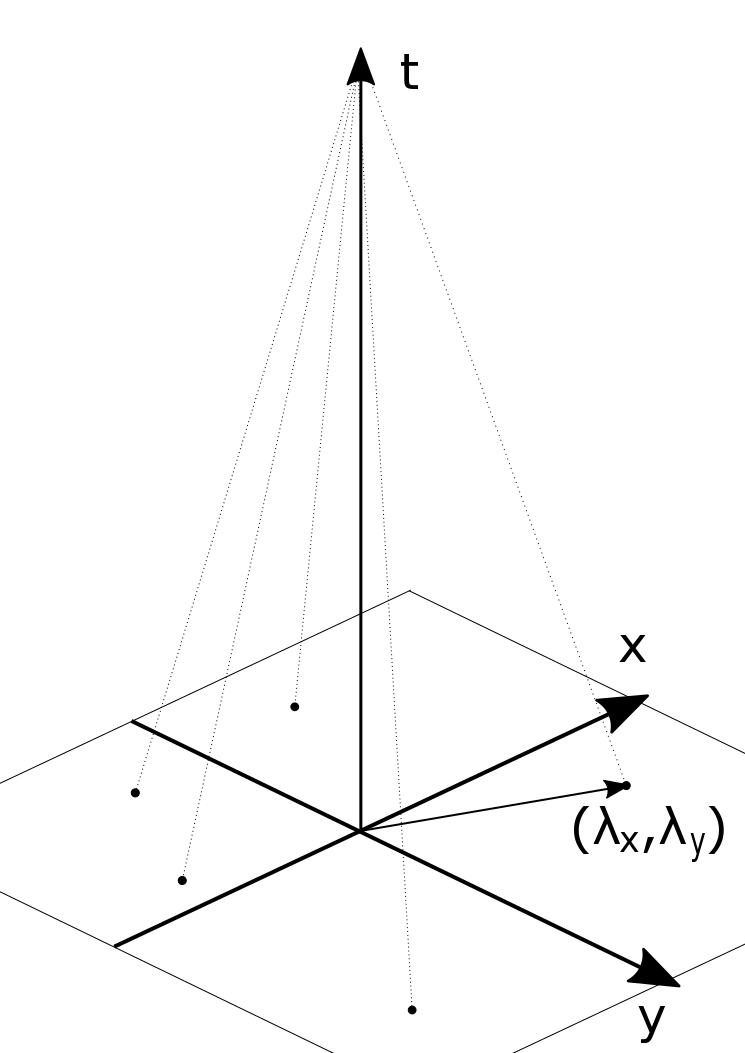
\includegraphics[scale=0.14]{algr}
		\captionsetup{labelformat=empty}
		\caption{Схема алгоритма}
	\end{figure}
		\end{minipage}
		\hfill
		\begin{minipage}{0.49\textwidth}
			Рассмотрим подробнее случай 2 пространственных переменных
	\begin{itemize}
		\item $\lambda = ({\lambda } ^{k_1}, {\lambda } ^{k_2})$ - все комбинации пар собственных чисел матриц $A_1, A_2$ соответственно
		\item опускаем прямые вида $x - \lambda dt$
		\item ${\bf{C}}^{k_1 k_2}$ - на основе решения, полученного в статье
	\end{itemize}
		\end{minipage}
	\end{figure}
	\begin{equation*}
	{{\bf{u}} ({\bf{x^*}}, t + dt)}
	= 
	\sum\limits_{k_1, k_2}^{} {{\bf{C}}^{k_1 k_2}{\bf{u}}_0 \left( { {x^*_1}- {\bf{\lambda }} ^{{k_1}}dt,{x^*_2} - {\bf{\lambda }} ^{{k_2}}dt} \right)}
	\end{equation*}
\end{frame}	

\begin{frame}\frametitle{Вычислительный алгоритм}
	\begin{itemize}
\item приближенное решение задачи Римана в момент времени $t = t + \delta t$, основываясь на начальных данных в некоторой окрестности. 

\item достаточно знать значения в локальной окрестности на предыдущем временном слое. 

\item восстанавливаем решение в каждой ячейке с помощью интерполяции
\end{itemize}
\end{frame}	

\begin{frame}\frametitle{Система уравнений упругой динамики}
	\begin{eqnarray*} \label{eq:1_2}
		\frac{\partial}{\partial t} \sigma_{1\:1} - (\lambda+2\mu) \frac{\partial}{\partial x_{1}} v_{1} - \lambda \frac{\partial}{\partial x_{2}} v_{2} = 0, \nonumber
		\\
		\frac{\partial}{\partial t} \sigma_{2\:2} - \lambda \frac{\partial}{\partial x_{1}} v_{1} - (\lambda+2\mu) \frac{\partial}{\partial x_{2}} v_{2} = 0, \nonumber
		\\
		\frac{\partial}{\partial t} \sigma_{1\:2} - \mu \frac{\partial}{\partial x_{1}} v_{2} - \mu \frac{\partial}{\partial x_{2}} v_{1} = 0, 
		\\
		\rho \frac{\partial}{\partial t} v_{1} - \frac{\partial}{\partial x_{1}} \sigma_{1\:1} - \frac{\partial}{\partial x_{2}} \sigma_{1\:2} = 0, \nonumber
		\\
		\rho \frac{\partial}{\partial t} v_{2} - \frac{\partial}{\partial x_{1}} \sigma_{1\:2} - \frac{\partial}{\partial x_{2}} \sigma_{2\:2} = 0, \nonumber
	\end{eqnarray*}
	
	где $ \lambda $ и $ \mu $ коэффициенты Ламе, $ \rho $ масовая плотность среды, $ \sigma_{1\:1} $, $ \sigma_{2\:2} $, $ \sigma_{1\:2} $ компоненты тензора напряжений, $ v_{1} $, $ v_{2} $ компоненты вектора скорости смещений.
\end{frame}

\begin{frame}\frametitle{Система уравнений упругой динамики}
	Введем вектор переменных $ \mathbf{u}=(\sigma_{1\:1}, \sigma_{2\:2}, \sigma_{1\:2}, v_{1}, v_{2})^{T} $.
	
	Тогда можно записать систему в виде:
	\begin{equation*} 
	\frac{{\partial {\mathbf{u}}\left( {t,{\mathbf{x}}} \right)}}{{\partial t}} +
	{{\mathbf{A}_1} \frac{{\partial {\mathbf{u}}\left( {t,{\mathbf{x}}}
				\right)}}{{\partial {x_1}}}}  + {{\mathbf{A}_2} \frac{{\partial {\mathbf{u}}\left( {t,{\mathbf{x}}}
				\right)}}{{\partial {x_2}}}} = {\mathbf{0}}
	\end{equation*}
\end{frame}

\begin{frame}\frametitle{Верификация алгорима}
	\begin{itemize}
		\item выявлено количественное совпадение решений задачи о распаде разрыва с аналитическим решением
	\end{itemize}
	\begin{figure}[ht!]
		\centering
		\begin{minipage}{0.5\textwidth}
			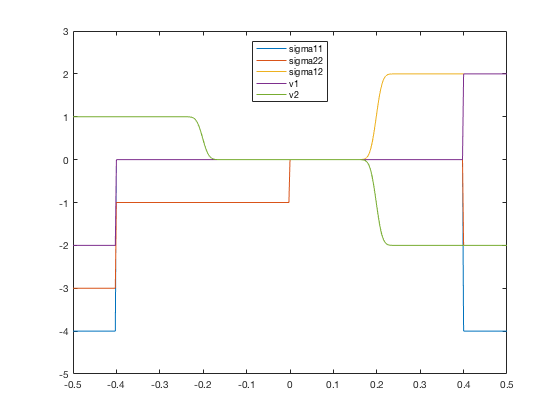
\includegraphics[width=\textwidth]{graph_test}
			\captionsetup{labelformat=empty}
			\caption{Приближенное решение}
		\end{minipage}
		\hfill
		\begin{minipage}{0.49\textwidth}
			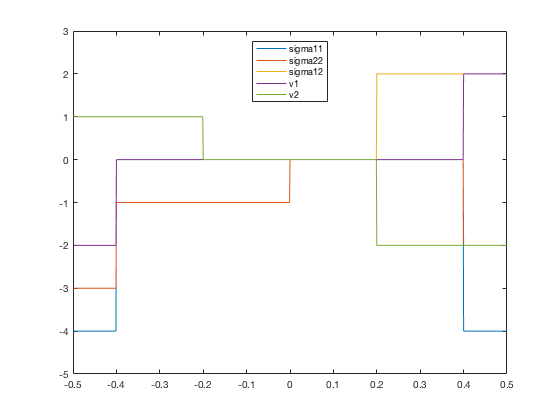
\includegraphics[width=\textwidth]{test_analyt}
			\captionsetup{labelformat=empty}
			\caption{Аналитическое решение}
		\end{minipage}
	\end{figure}
\end{frame}	

\begin{frame}\frametitle{Верификация алгорима}
	
	\begin{itemize}
		\small
		\item показана сеточная сходимость численного метода на модельной задаче (аппроксимация второго порядка по пространству)
			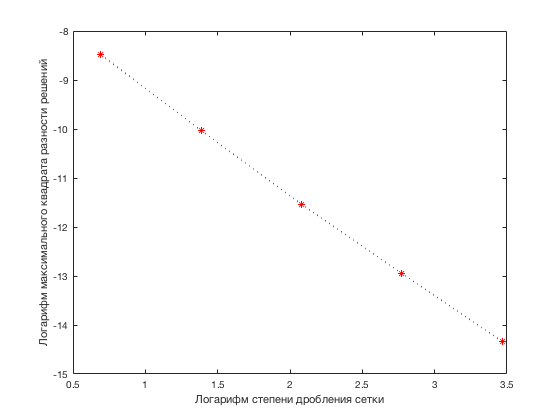
\includegraphics[scale=0.45]{shod.png}
	\end{itemize}
\end{frame}	

\subsection{Вычислительные эксперименты (примеры)}

\begin{frame}\frametitle{Вычислительный эксперимент}
	\footnotesize
Рассмотрена задача распространения упругих вибраций внутрь нефтеносного пласта
	\begin{figure}[ht!]
		\centering
		\begin{minipage}{0.5\textwidth}
			\centering
		\includegraphics[scale=0.2]{area}
		\end{minipage}
		\hfill
		\begin{minipage}{0.49\textwidth}
	\begin{itemize}
		\footnotesize
		\item Для задачи взяты параметры, соответсвующие некоторым реальным типам геологических пород
		
		\item Расчетная область имеет размер 60м х 600м
		
		\item Скорость распространения волны порядка 1000м/с
		
		\item На поверхности установлен источник, дающий возмущения с указанной частотой 
		
		\item На внутренних границах задаются либо условия проскальзывания, либо условия слипания
	\end{itemize}
		\end{minipage}
	\end{figure}

\end{frame}

\begin{frame}\frametitle{Вычислительный алгоритм}
	В реализации алгоритма использовались условия на границах:\guillemotleft{}условия полного слипания\guillemotright{} или \guillemotleft{}условия проскальзывания без
	трения\guillemotright{}
	\begin{equation*} 
	\begin{split}
	v_{1} \left( t, \,{\mathbf{x}} \in \Gamma^- \right) &= v_{1} \left( t, \,{\mathbf{x}} \in \Gamma^+ \right) \nonumber
	\\
	v_{2} \left( t, \,{\mathbf{x}} \in \Gamma^- \right) &= v_{2} \left( t, \,{\mathbf{x}} \in \Gamma^+ \right) \nonumber
	\\
	\sigma_{1\:1} \left( t, \,{\mathbf{x}} \in \Gamma^- \right) &= \sigma_{1\:1} \left( t, \,{\mathbf{x}} \in \Gamma^+ \right) 
	\\
	\sigma_{1\:2} \left( t, \,{\mathbf{x}} \in \Gamma^- \right) &= \sigma_{1\:2} \left( t, \,{\mathbf{x}} \in \Gamma^+ \right) \nonumber
	\end{split}
	\quad
	\begin{split}
	v_{1} \left( t, \,{\mathbf{x}} \in \Gamma^- \right) = v_{1} \left( t, \,{\mathbf{x}} \in \Gamma^+ \right) \nonumber
	\\
	\sigma_{1\:1} \left( t, \,{\mathbf{x}} \in \Gamma^- \right) = \sigma_{1\:1} \left( t, \,{\mathbf{x}} \in \Gamma^+ \right) 
	\\
	\sigma_{1\:2} \left( t, \,{\mathbf{x}} \in \Gamma^- \right) = 0 \nonumber
	\\
	\sigma_{1\:2} \left( t, \,{\mathbf{x}} \in \Gamma^+ \right) = 0 \nonumber
	\end{split}
	\end{equation*}
\end{frame}


\begin{frame}\frametitle{Вычислительный эксперимент}

	Результаты показали 
	\begin{itemize}
		\item Проскальзывающая внутренняя граница ведет себя как стенка волновода
	\end{itemize}
	
	\begin{figure}[ht!]
		\centering
		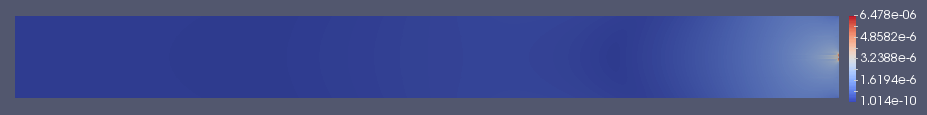
\includegraphics[scale=0.346]{adhes}\\
		\medskip
		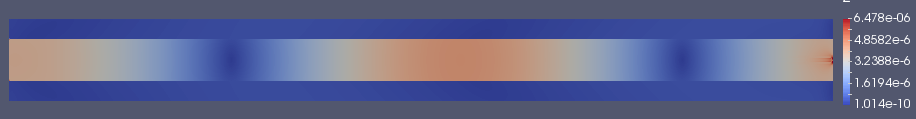
\includegraphics[scale=0.35]{sliding10}
	\end{figure}
	
\end{frame}

\begin{frame}\frametitle{Вычислительный эксперимент}
	Результаты показали 
	\begin{itemize}
		\item При увеличении частоты (при уменьшении длины волны до характерного размера расстояния между внутренними трещинами) область с проскальзывающими границами ведет себя как однородная. 
	\end{itemize}
	
	\begin{figure}[ht!]
		\centering
		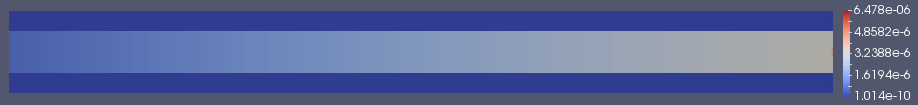
\includegraphics[scale=0.346]{sliding1}\\
		\pause
		\medskip
		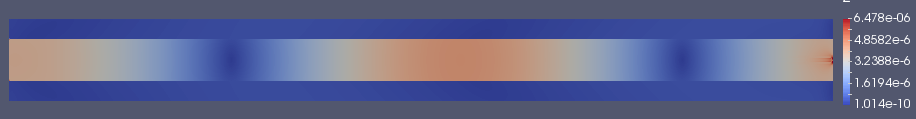
\includegraphics[scale=0.346]{sliding10}\\
		\pause
				\medskip
				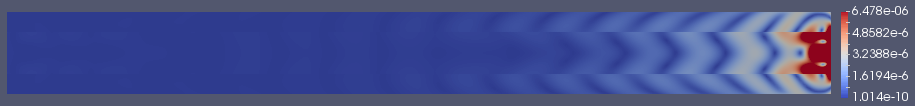
\includegraphics[scale=0.346]{sliding100}\\
	\end{figure}
	
\end{frame}

\section{Заключение}

\begin{frame}\frametitle{Заключение}
	\small
Построен вычислительный алгоритм решения начально-краевой задачи для гиперболической системы линейных дифференциальных уравнений 1 порядка на основании приведенного в статье решения задачи Римана
\pause
\begin{enumerate} 
	\item {алгоритм верифицирован на ряде тестов}
	\pause
	\item {хорошее быстродействие алгоритма еще до распараллеливания}
	\pause
	\item {применим к задаче любой размерности}
	\pause
	\item {имеет большой потенциал к распараллеливанию}
	\begin{enumerate} 
	\item {Решение в каждом узле вычисляется независимо}
	\item {Построение интерполяционного полинома строится независимо на каждом интервале}
	\end{enumerate} 
	\pause
	\item рассмотрена задача распространения возмущений источника в среде с внутренними границами и показано, что при определенных условиях на этих границах (условия проскальзывания) эти возмущения доставлены на глубину без существенного рассеивания
\end{enumerate} 

Результаты работы изложены в статье, которая готовится к изданию.
\end{frame}


\begin{frame}[plain]
  \begin{center}
  {\Huge Спасибо за внимание!}
  \vspace{8ex}

  Мазепов Виталий

  e-mail: \colorhref{mailto:mazepov@phystech.edu}{mazepov@phystech.edu}
  \end{center}
\end{frame}


\end{document}
